\section{Выбор и обоснование структурной схемы (алгоритма работы) проектируемой системы}

\subsection{Обоснование общей архитектуры программного комплекса}

Проектируемая система реализует гибридный асимметричный алгоритм сжатия и восстановления цифровых изображений, сочетающий классические методы цифровой обработки сигналов (DSP) и технологии глубокого машинного обучения (Deep Learning). В основу системы положена клиент-серверная архитектура, реализующая концепцию Edge-to-Cloud Offloading.

Данная архитектура позволяет перенести основную вычислительную нагрузку с маломощного устройства-отправителя (Edge) на высокопроизводительный сервер (Cloud). Структурная схема системы, отражающая взаимодействие модулей и потоки данных, представлена на рисунке~\ref{fig:structural_scheme}.

\begin{figure}[ht]
    \centering
    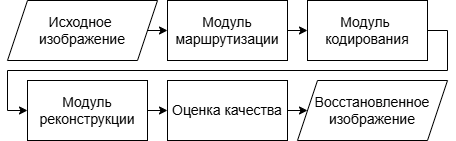
\includegraphics[width=0.9\textwidth]{media/images/structural_scheme.png}
    \caption{Структурная схема гибридного программного комплекса}
    \label{fig:structural_scheme}
\end{figure}

Функциональный состав системы включает:
\begin{enumerate}
    \item Модуль адаптивной маршрутизации (Smart Router): выполняет первичный анализ метаданных файла (размер, разрешение) и выбирает оптимальный путь обработки (Pass-Through или Hybrid Compression).
    \item Модуль вейвлет-кодирования: реализует дискретное вейвлет-преобразование (DWT) Хаара для получения низкочастотной аппроксимации изображения, которая служит каркасом для передачи.
    \item Модуль экстракции метаданных: извлекает семантические дескрипторы (цветовую палитру и карту границ Кенни \cite{canny1986}), которые весят единицы килобайт, но критически важны для предотвращения нейросетевых искажений.
    \item Модуль нейросетевого синтеза: на стороне приемника выполняет тензорный инференс моделей ESPCN \cite{shi2016} или FSRCNN \cite{dong2016fsrcnn}, восстанавливая текстуры и детали.
    \item Модуль постобработки и рекомбинации: выполняет слияние алгоритмического результата с метаданными в цветовом пространстве YCrCb для коррекции яркости и контраста.
\end{enumerate}

\subsection{Алгоритм работы модуля адаптивной маршрутизации и кодирования}

Процесс кодирования спроектирован как последовательность легковесных операций, не требующих наличия графического процессора (GPU) на стороне отправителя. Логика работы кодера представлена на рисунке~\ref{fig:encoder_algorithm}.

\begin{figure}[ht]
    \centering
    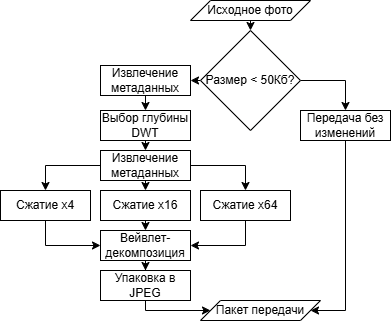
\includegraphics[width=0.7\textwidth]{media/images/encoder_algorithm.png}
    \caption{Схема алгоритма адаптивной маршрутизации и кодирования}
    \label{fig:encoder_algorithm}
\end{figure}

Критическими этапами кодирования являются:
\begin{enumerate}
    \item Пороговая фильтрация: если объем данных мал (менее 50 Кбайт), алгоритм игнорирует сжатие, предотвращая ситуацию, когда метаданные весят больше самого изображения.
    \item Экстракция структурных контуров: для фиксации границ объектов используется детектор Кенни \cite{canny1986}. Процесс включает гауссово размытие, вычисление градиента яркости оператором Собеля, подавление не-максимумов и двойную пороговую фильтрацию. Это необходимо, так как нейросети склонны размывать резкие границы при масштабировании.
    \item Децимация через DWT: вместо простого изменения размера используется вейвлет-аппроксимация (LL-субполоса). Это математически гарантирует сохранение средней яркости и энергетического баланса кадра, что важно для метрики PSNR.
    \item Контейнеризация: упаковывание вейвлет-скелета в формат JPEG позволяет использовать эффективное энтропийное кодирование (алгоритм Хаффмана) для финального уменьшения объема передаваемых байтов. При этом учитывается, что стандартный переход в цветовое пространство YCbCr и субдискретизация хроматических каналов (4:2:0) вносят искажения в яркостную составляющую, что требует последующей компенсации.
\end{enumerate}

\subsection{Алгоритм работы модуля нейросетевой реконструкции}

Модуль реконструкции выполняет наиболее ресурсоемкую часть работы, используя предобученные сверточные нейронные сети. Алгоритм декодирования представлен на рисунке~\ref{fig:decoder_algorithm}.

\begin{figure}[ht]
    \centering
    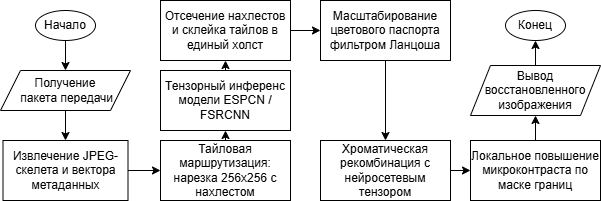
\includegraphics[width=0.8\textwidth]{media/images/decoder_algorithm.png}
    \caption{Схема алгоритма нейросетевой реконструкции и постобработки}
    \label{fig:decoder_algorithm}
\end{figure}

Технологические особенности процесса реконструкции:
\begin{enumerate}
    \item Адаптивный выбор модели: система анализирует визуальную сложность входного кадра через дисперсию оператора Лапласиана. При высокой детализации используется модель FSRCNN \cite{dong2016fsrcnn} с глубокой архитектурой, при низком шуме — модель ESPCN \cite{shi2016}, использующая эффективную субпиксельную свертку (PixelShuffle).
    \item Механизм тайловой маршрутизации (Overlapping Tiling): для обработки изображений высокого разрешения на ограниченных ресурсах оперативной памяти применяется нарезка на блоки. Нахлест в 16 пикселей позволяет нейросети учитывать контекст соседних областей, исключая возникновение видимых швов на границах блоков.
    \item Коррекция в пространстве YCrCb: из-за необратимых потерь в JPEG-контейнере восстановленное изображение может потерять исходную яркость и контраст. Алгоритм переводит результат в пространство YCrCb, где канал яркости (Y) корректируется по оригинальному цветовому паспорту с использованием переноса статистических моментов (алгоритм Рейнхарда \cite{reinhard2001}).
    \item Контурно-зависимое повышение резкости: фильтр нерезкой маски (Unsharp Mask) применяется не ко всему кадру, а только к зонам, указанным в карте границ Кенни. Это позволяет избежать усиления шума на гладких поверхностях, сохраняя резкость границ объектов.
\end{enumerate}

\subsection{Алгоритм оценки качества и профилирования}

Заключительный этап работы системы — объективный контроль качества. Алгоритм сопоставляет оригинальное и восстановленное изображения по следующим критериям:
\begin{enumerate}
    \item PSNR (Peak Signal-to-Noise Ratio): определяет логарифмическую меру искажений на уровне пикселей. Значения свыше 30 дБ считаются нормой для систем связи.
    \item SSIM (Structural Similarity Index) \cite{wang2004ssim}: оценивает сохранность структурных паттернов. В отличие от PSNR, эта метрика лучше коррелирует с человеческим восприятием качества.
    \item Профилирование асимметрии: система фиксирует время кодирования и декодирования. Успешным считается результат, при котором время реконструкции на сервере многократно превышает время сжатия на клиенте, что подтверждает эффективность переноса нагрузки.
\end{enumerate}